%%%%%%%%%%%%%%%%%%%%%%%%%%%%%%%%%%%%%%%%%%%%%%%%%%%%%%%%%%%%%%%%%%%%%%
% amspaper.tex --  LaTeX-based template for submissions to American 
% Meteorological Society journals
%
% Template developed by Amy Hendrickson, 2013, TeXnology Inc., 
% amyh@texnology.com, http://www.texnology.com
% following earlier work by Brian Papa, American Meteorological Society
%
% Email questions to latex@ametsoc.org.
%
%%%%%%%%%%%%%%%%%%%%%%%%%%%%%%%%%%%%%%%%%%%%%%%%%%%%%%%%%%%%%%%%%%%%%
% PREAMBLE
%%%%%%%%%%%%%%%%%%%%%%%%%%%%%%%%%%%%%%%%%%%%%%%%%%%%%%%%%%%%%%%%%%%%%

%% Start with one of the following:
% DOUBLE-SPACED VERSION FOR SUBMISSION TO THE AMS
\documentclass{ametsoc}

% TWO-COLUMN JOURNAL PAGE LAYOUT---FOR AUTHOR USE ONLY
% \documentclass[twocol]{ametsoc} 

%%%%%%%%%%%%%%%%%%%%%%%%%%%%%%%%
%%% To be entered only if twocol option is used

\journal{jamc}

\usepackage{amsmath}
\usepackage{amssymb}
\usepackage{wasysym}

%  Please choose a journal abbreviation to use above from the following list:
% 
%   jamc     (Journal of Applied Meteorology and Climatology)
%   jtech     (Journal of Atmospheric and Oceanic Technology)
%   jhm      (Journal of Hydrometeorology)
%   jpo     (Journal of Physical Oceanography)
%   jas      (Journal of Atmospheric Sciences)	
%   jcli      (Journal of Climate)
%   mwr      (Monthly Weather Review)
%   wcas      (Weather, Climate, and Society)
%   waf       (Weather and Forecasting)
%   bams (Bulletin of the American Meteorological Society)
%   ei    (Earth Interactions)

%%%%%%%%%%%%%%%%%%%%%%%%%%%%%%%%
%Citations should be of the form ``author year''  not ``author, year''
\bibpunct{(}{)}{;}{a}{}{,}

%%%%%%%%%%%%%%%%%%%%%%%%%%%%%%%%

%%% To be entered by author:

%% May use \\ to break lines in title:

\title{Role of forcing scale on $\beta$-plane turbulence: jet formation}

%%% Enter authors' names, as you see in this example:
%%% Use \correspondingauthor{} and \thanks{Current Affiliation:...}
%%% immediately following the appropriate author.
%%%
%%% Note that the \correspondingauthor{} command is NECESSARY.
%%% The \thanks{} commands are OPTIONAL.

\authors{Junyi Chai\correspondingauthor{Junyi Chai, Bellevue, WA 98004}
\thanks{Current affiliation: MSFT}}
\affiliation{Atmospheric and Oceanic Sciences Program, Princeton University, Princeton, New Jersey}
\email{junyi.x.chai@gmail.com}
\extraauthor{Malte Jansen}
\extraaffil{Department of the Geophysical Sciences, University of Chicago, Chicago, Illinois}


%%%%%%%%%%%%%%%%%%%%%%%%%%%%%%%%%%%%%%%%%%%%%%%%%%%%%%%%%%%%%%%%%%%%%
% ABSTRACT
%
% Enter your Abstract here

\abstract{Turbulence regimes are examined in forced-dissipative, two-dimensional
flow on $\beta$-plane with particular emphasis on jet formation.
Two scales have been known to distinguish the flow from an isotropic
turbulence: the Rhines wavenumber $k_{Rh}=\sqrt{\beta/2U_{rms}}$
and the turbulence-wave crossover wavenumber $k_{\varepsilon}=\mathcal{\mathcal{C}_{\varepsilon}}\beta^{3/5}\varepsilon^{-1/5}$;
here $U$ is r.m.s. velocity, $\beta$ is planetary potential vorticity
gradient, $\mathcal{\mathcal{C}_{\varepsilon}}$ is a constant of
about 0.5$\sim$0.6, and $\varepsilon$ is the upscale energy flux
rate. The anisotropy of the flow is known to be largely determined
by the zonostrophic index $Z=k_{\varepsilon}/k_{Rh}$. In this study,
it is shown that the forcing scale $k_{f}^{-1}$ also influences the
anisotropy, especially when it is comparable to or even smaller than
the crossover scale $k_{\varepsilon}^{-1}$. The role of forcing scale
is conveniently characterized by the ratio $\Pi=k_{f}/k_{\varepsilon}$.
When $\Pi<1$, the crossover wavenumber is in the enstrophy cascade range
and a new form is proposed as $k_{\varepsilon}\Pi^{-2/3}$, indicating
a wider range of scales under $\beta$-effect than that would be predicted
from $Z$ alone. Turbulence regimes are explored in $(Z,\Pi)$ space
with numerical simulations. When $1.5\apprle Z\apprle2.5$, $Z$ and
$\Pi$ both influence jet formation: jets are stronger and more coherent
for larger $Z$ or smaller $\Pi$. When $Z\apprge2.5$, the flow are
dominated by strong jets. This regime has previously been characterized
as the zonostrophic turbulence for $\Pi\apprge4$. When $\Pi$ decreases,
the flow gradually transits into a new turbulence regime at $\Pi\apprle1$.
This regime is ``quasi-linear'' in the sense that eddy-eddy interactions
are negligible while eddy/mean-flow interactions dominate the nonlinear
energy and enstrophy transfers. Energy injected at the forcing scale
is directly transfered into the jets at the largest scale. The flow
with zonal-mean potential vorticity similar to a staircase structure
is approached in the corner of the quasi-linear regime when the zonostrophic
index is very high ($Z\apprge7$). The values of $\Pi$ are estimated
for Earth's atmosphere and oceans.} 

\begin{document}


%% Necessary!
\maketitle


%%%%%%%%%%%%%%%%%%%%%%%%%%%%%%%%%%%%%%%%%%%%%%%%%%%%%%%%%%%%%%%%%%%%%
% MAIN BODY OF PAPER
%%%%%%%%%%%%%%%%%%%%%%%%%%%%%%%%%%%%%%%%%%%%%%%%%%%%%%%%%%%%%%%%%%%%%
%
\section{Introduction}

Planetary rotation profoundly determines the macroturbulence in the
atmosphere and ocean, distinguishing it from the flows at much smaller
scales in two different ways. First, the large scale flow is in near
geostrophic balance due to the rotation. Therefore macroturbulence
is quasi- two-dimensional in nature, which fundamentally changes the
picture for nonlinear energy transfer \citep{Kraichnan1967,Charney1971},
predictability \citep{Leith1971,Leith1972}, and tracer transport/mixing
\citep{Batchelor1959,Shuckburgh2003} from its three-dimensional counterpart.
Second, the differential rotation on a sphere, or $\beta$-effect,
introduces anisotropy to the flow. As a result, zonal jets spontaneously
form, and the flow is rather an interplay of turbulence, Rossby waves
and jets. Arguably, the simplest idealization to study the macroturbulence
with both effects of planetary rotation is a forced-dissipated two-dimensional
(2d) flow on a $\beta$-plane. This idealization contains the complexity
of nonlinear interactions, yet it is fully determined by a handful
of factors: forcing, dissipation (of both energy and enstrophy) and
$\beta$-effect. In this idealized setting, it is promising to chart
different turbulent regimes using a few nondimensional numbers.
These turbulent regimes have their correspondence in the real geophysical
flows, as well as in models with increased complexity. Understanding
these regimes will be a first step towards a general circulation theory.

One nondimensional number that is well-known to determine the anisotropy
of the flow is the ratio between two length scales: the Rhines scale
and the turbulence-wave crossover scale. The Rhines scale
may be considered as the jet scale, which in terms of wavenumber is
\begin{equation}
    k_{Rh}=(\beta/2U_{rms})^{1/2},\label{eq:Rhines_wavenumber_beta_Urms}
\end{equation}
where $U_{rms}$ is the rms velocity of the whole flow \citep{Rhines1975}.
\footnote{The form and meaning of Rhines scale have been
under debate since it has been proposed. In some studies, rms velocity
of the eddies or the meridional wind has been used, while the Rhines scale itself
has been used as an estimate for either eddy scale, jet scale, or
the scale where energy gets channeled into jets \citep{Williams1978,Jansen2012,Chai2014,Liu2015,Chemke2015}.
Here we choose the definition that is consistent with zonostrophic turbulence.}
The turbulence-wave crossover scale marks the transition from
isotropic eddies to Rossby waves, which in term of wavenumber is
\begin{equation}
    k_{\varepsilon}=\mathcal{C}_{\varepsilon}\beta^{3/5}\varepsilon^{-1/5},\label{eq:classical_crossover_wavenumber}
\end{equation}
where $\varepsilon$ is the upscale energy flux and $\mathcal{C}_{\varepsilon}$ is a constant of about
$0.5\sim0.6$ \citep{Vallis1993,Galperin2010,Smith2002}. It is thought that
eddies smaller than the crossover scale are only weakly influenced by the 
$\beta$-effect, therefore behaving as isotropic turbulence, whereas eddies 
larger than the crossover scale predominately behave as Rossby waves.

Intuitively, the ratio of the two scales
\begin{equation}
    Z=k_{\varepsilon}/k_{Rh},\label{eq:zonostrophic_index_def}
\end{equation}
determines whether jets form or not, strong or weak, as the larger
$Z$ is, the larger range of scales of eddies will become Rossby waves, whose
unique dispersion relation strongly modifies their energy transfer in a way 
that most of the energy is directed into the zonal modes (a simple explanation 
is given by \citeauthor{Vallis1993}
{[}1993{]}; another explanation exploring a new invariant unique for
Rossby waves is given by \nocite{Balk1991,Balk2005}Balk {[}1991,
2005{]}, \citeauthor{Nazarenko2009} {[}2009{]}).
Specifically, \citet{Galperin2010}
divide $\beta$-plane turbulence into two regimes based on $Z$ -- \textit{zonostrophic}
regime for $Z\gtrsim2.5$ and \textit{friction-dominated} regime
for $Z\lesssim1.5$ -- and the transition between them. 
And $Z$ is coined as the \textit{zonostrophic
index}. Zonostrophic turbulence gets its name because the flow
is dominated by strong zonal jets. Whereas in the friction-dominated
regime, the inverse energy cascade is halted by friction before reaching the 
crossover scale and thus the flow is close to isotropic turbulence.

Quantitatively, the energy spectra of eddies and zonal flow for the
zonostrophic turbulence, as 
illustrated in Fig. \ref{EKE_KE_spectra_illustrate}, further
explain how the zonostrophic index $Z$ set the anisotropy of the flow. 
Let the 2d flow be stirred by a spectrally localized forcing at a (high) wavenumber $k_{f}$.
The eddies keeps the same the energy spectrum as the isotropic turbulence,
with an energy inverse cascade branch ($k<k_f$) as 
\begin{equation}
    \mathcal{E}(k)=\mathcal{C_{K}}\varepsilon^{2/3}k^{-5/3}\label{eq:Kolmogorov_Kraichnan_spectrum_energy}
\end{equation}
and a steeper enstrophy direct cascade branch ($k>k_f$) as
\begin{equation}
    \mathcal{E}(k)=\mathcal{C'_{K}}\eta^{2/3}k^{-3},\label{eq:Kolmogorov_Kraichnan_spectrum_enstrophy}
\end{equation}
where $\varepsilon$ and $\eta$ are the upscale energy flux and downscale enstrophy
flux respectively; $\mathcal{C_{K}}$ and $\mathcal{C'_{K}}$ are the Kolmogorov constants
of about $6\sim7$ and $1.3\sim1.6$ respectively\citep{Maltrud1991,Smith1993,Paret1997,Chen2006,Borue1993,Gotoh1998}.
The central piece of zonostrophic turbulence is that 
energy in the zonal modes (jets) follows a universal spectrum determined
by $\beta$ and wavenumber as
\begin{equation}
\mathcal{E_{Z}}(k)=\mathcal{C_{Z}}\beta^{2}k^{-5},\ k_{x}=0,\label{eq:zonostrophic_spectrum}
\end{equation}
where $k_{x}$ is the zonal wavenumber, and the constant $\mathcal{C_{Z}}$
is found to be about 0.5 \citep{Sukoriansky2002,Smith2002,Galperin2010}.
Such spectrum has been observed in many numerical simulations 
\citep{Chekhlov1996,Smith2002,Huang2001,Sukoriansky2002,Sukoriansky2007},
more or less in the Jovian atmosphere \citep{Sukoriansky2002,Choi2011,Galperin2014}
and even in high-resolution ocean simulations \citep{Galperin2004}.
Zonal and eddy kinetic spectra intersect at the crossover wavenumber $k_{\varepsilon}$.
Eventually, friction comes into effect and halts the energy cascade at jet scale $k_r^{-1}$,
which is close to the Rhines scale.\footnote{The zonal spectrum (\ref{eq:zonostrophic_spectrum})
also lays Rhines scale on a quantitative ground, as by assuming
most energy is in the jets and an integration of (\ref{eq:zonostrophic_spectrum}) 
from $k_{r}$ to $\infty$ we can get $k_{r}\simeq1.2k_{Rh}$.}
As when inverse cascade proceeds beyond the crossover scale ($k<k_\varepsilon$), 
the zonal mode contains more and more energy compared to eddies,
clearly the larger $Z$ is, the more percentage of energy will be in the jets.

The above zonostrophic turbulence picture and the derivation of
crossover scale in (\ref{eq:classical_crossover_wavenumber}) assume
that the forcing scale is much smaller than the crossover scale so that
there exists an extended inverse cascade range in between.
The details of the forcing, including the forcing scale,
may lose their influence on the large scale flow due to
the locality hypothesis. This is probably true when $k_{f}/k_{\varepsilon}\apprge4$,
which is noted by \citet{Sukoriansky2007} as a prerequisite
to reach zonostrophic turbulence and is due to the fact
that the inverse cascade is only weakly local in scale: 
energy flux across scale $l$ involves
the thinning of subscale eddies 4 to 8 times smaller than $l$ by
the strain at $l$ \citep{Chen2006}.
The condition $k_{f}/k_{\varepsilon}\apprge4$, however, 
is rarely satisfied in many real geophysical flows, 
for example, in the Earth's atmosphere \citep{Schneider2006,Merlis2009}
and oceans \citep{Tulloch2011}. In this case, the details of
forcing is not likely to be negligible. Furturemore, literature 
on potential vorticity (PV) staircase hints that
forcing scale itself may play an important role 
in jet formation when it is comparable to crossover scale.
PV staircase has long been hypothesized
as a model for jet formation, which is the limiting case that PV is
perfectly mixed between jets while having distinct jumps at the center
of jets \citep{Marcus1993,Marcus1998,Dunkerton2008,Dritschel2008}.
The flow with a near-perfect PV staircase structure has been recently 
simulated by \citet{Scott2012}. Although \citet{Scott2012} suggest the very high
zonostrophic index as the key to obtain the PV staircase, examining
their experiment setup, our calculation suggests that 
$k_{f}/k_{\varepsilon}<1$, which may be the additional criterion
to get PV staircase.
\footnote{In a later study, \citet{Scott2012a} suggest that PV staircase can
easily form when the forcing scale is as large as the jet scale and
$k_{f}/k_{\varepsilon}\apprle1/6$, which is more extreme than the
condition we suggest here. This extreme regime is reached by a rather
unusual topographic forcing without large scale friction, which makes
it not straightforward to compare with the forced-dissipative turbulence
in this study.} 

In this study, we aim to answer how the forcing scale influences the
flow. From the above discussion, the ratio
\begin{equation}
\Pi=k_{f}/k_{\varepsilon}\label{eq:def_Pi_index}
\end{equation}
suggests itself as an important nondimensional number to characterize
the role of the forcing scale. When $\Pi<1$, the scale $k_{\varepsilon}^{-1}$
is now within the direct enstrophy cascade range and therefore formulation
of turbulence-wave crossover scale in (\ref{eq:classical_crossover_wavenumber})
should no longer hold. This paper is organized
as followings. In section 2, we derive a new crossover scale in the
enstrophy cascade branch for $\Pi<1$. In section 3, a set of experiments
varying both $\Pi$ and $Z$ are carried out. Experiment results are
analyzed in section 4, which are understood using turbulent phenomenology
and our new crossover scale. In section 5, we conclude with an updated
chart for turbulence regimes in the ($Z$, $\Pi$) space and discuss
its relevance with the observed geophysical flows.


\section{Theory}

Consider the first case where $\beta$-effect does not affect the flow at the forcing
scale so that the classical dual cascades extend from the forcing
wavenumber $k_{f}$. Energy inversely cascades to larger scales and
enstrophy directly cascades to smaller scales. The inverse of eddy
turnover time defines a strain rate, or ``turbulence frequency''
$\omega_{t}$, consisting of two branches: an inverse energy cascade
branch for $k<k_{f}$ and a direct enstrophy cascade branch for $k>k_{f}$.
From dimensional analysis, the turbulence frequency in the inverse
energy cascade branch is
\begin{equation}
\omega_{t}=\mathcal{C}_{\omega,\varepsilon}\varepsilon^{1/3}k^{2/3},\label{eq:eddy_turnover_freq_inverse_cascade}
\end{equation}
and in the direct enstrophy cascade branch is
\begin{equation}
\omega_{t}=\mathcal{C}_{\omega,\eta}\eta^{1/3},\label{eq:eddy_turnover_freq_direct_enstrophy_cascade}
\end{equation}
where $\mathcal{C}_{\omega,\varepsilon}$ and $\mathcal{C}_{\omega,\eta}$
are universal constants. If the forcing scale is well localized, enstrophy
flux is related to energy flux by

\begin{equation}
\eta=k_{f}^{2}\varepsilon.\label{eq:energy_enstrophy_flux_relationship}
\end{equation}
As $\omega_{e}$ must be continuous across $k_{f}$, we have

\[
\mathcal{C}_{\omega,\varepsilon}\varepsilon^{1/3}k_{f}^{2/3}=\mathcal{C}_{\omega,\eta}\eta^{1/3}.
\]
Using the relation (\ref{eq:energy_enstrophy_flux_relationship}),
we relate the two constants as $\mathcal{C}_{\omega,\varepsilon}=\mathcal{C}_{\omega,\eta}$.
Therefore, a general form for $\omega_{t}$ can be written as

\begin{equation}
\omega_{t}=\mathcal{C}_{\omega,\varepsilon}\varepsilon^{1/3}\begin{cases}
k^{2/3}, & k<k_{f}\\
k_{f}^{2/3}, & k>k_{f}
\end{cases},\label{eq:eddy_turnover_freq_general_form}
\end{equation}
which is a monotonic function increasing with $k$.

The well-known Rossby wave frequency is 

\begin{equation}
\omega_{\beta}=-\frac{\beta k_{x}}{k^{2}}.\label{eq:Rossby_wave_freq_kx_k}
\end{equation}
As the crossover scale is at the isotropic turbulence boundary, we
take $k_{x}\sim k$ and the magnitude of Rossby wave frequency is

\begin{equation}
|\omega_{\beta}|\simeq\frac{\beta}{k}.\label{eq:Rossby_wave_freq_k}
\end{equation}
As illustrated in Fig. \ref{crossover_illustrate}, the classical
crossover wavenumber $k_{\varepsilon}$ is assumed to be the intersection
of the energy cascade branch of $\omega_{t}$ and $|\omega_{\beta}|$,
written as

\begin{equation}
k_{\varepsilon}=\mathcal{C}_{\omega,\varepsilon}^{-3/5}\beta^{3/5}\varepsilon^{-1/5}.\label{eq:crossover_k_energy_branch}
\end{equation}
However, it is also possible that the enstrophy cascade branch of
$\omega_{t}$ intersects $|\omega_{\beta}|$ at

\begin{equation}
k_{\eta}=\mathcal{C}_{\mathcal{K}}^{-1/2}\beta\varepsilon^{-1/3}k_{f}^{-2/3}.\label{eq:crossover_k_enstrophy_branch}
\end{equation}
The relationship between $k_{\varepsilon}$ and $k_{\eta}$ can be
seen clearly using the non-dimensional number $\Pi$ we proposed in
the introduction as

\begin{equation}
k_{\eta}=\Pi^{-2/3}k_{\varepsilon}.\label{eq:k_eta_k_epsilon_relation}
\end{equation}
As $|\omega_{\beta}|$ monotonically decreases with $k$ and $\omega_{t}$
monotonically increases with $k$, $\omega_{t}$ and $|\omega_{\beta}|$
will intersect at a unique wavenumber. We regard this wavenumber as
the generalized crossover wavenumber, denoted by $k_{\beta}$. As
seen from Fig. \ref{crossover_illustrate}, which branch of $\omega_{t}$
intersects with $|\omega_{\beta}|$ and therefore which one of $k_{\varepsilon}$
and $k_{\eta}$ gives the generalized crossover wavenumber $k_{\beta}$
can be conveniently determined by $\Pi$. If $\Pi>1$, the crossover
scale is within the energy cascade range, in which the formally evaluated
$k_{\eta}$ obeys

\[
k_{\eta}<k_{\varepsilon}=k_{\beta}<k_{f},
\]
and the classical crossover wavenumber keeps its meaning. If $\Pi<1$,
the crossover scale in now within the enstrophy cascade regime, and
we have

\[
k_{f}<k_{\varepsilon}<k_{\eta}=k_{\beta}.
\]
Now the classical crossover wavenumber loses its meaning. At $\Pi=1$,
all the three wavenumbers $k_{f}$, $k_{\varepsilon}$ and $k_{\eta}$
are identical. For both energy and enstrophy cascade ranges, the
generalized crossover wavenumber can be conveniently summarized as

\begin{equation}
k_{\beta}=\max(k_{\varepsilon},k_{\eta})=k_{\varepsilon}\max(1,\Pi^{-2/3}),\label{eq:generalized_crossover_wavenumber}
\end{equation}
where $\max(x,y)$ returns the larger one out of $x$ and $y$. 

The range of of scales influenced by the $\beta$-effect determines
how anisotropic the flow is. When $\Pi<1$, the classical scaling
$k_{\varepsilon}$ underestimates the generalized crossover wavenumber.
In this case, the zonostrophic index $Z$ underestimates the range
of scales under $\beta$-effect and thus underestimates the anisotropy
of the flow. Using the generalized crossover wavenumber $k_{\beta}$,
we may define a ``jet index'' to properly measure the width of the
range of scales under $\beta$-effect as

\begin{equation}
Z_{J}=\frac{k_{\beta}}{k_{Rh}}=\max(1,\Pi^{-2/3})Z.\label{eq:jet index}
\end{equation}
Here we assume that the Rhines scale still roughly gives the energy
halting scale, though the energy halting scale will inevitably have a
dependency on $\Pi$ as the universal spectrum (\ref{eq:zonostrophic_spectrum})
does not hold in the $\Pi<1$ regime. Using the jet index, we would
expect the jets to be even stronger if $\Pi$ is reduced to below 1 for
the same zonostrophic index. As an analogy of the transition between
friction-dominated and zonostrophic regimes based on $Z$, a more
general condition for jet formation may be that $Z_{J}$ be larger than a
critical value $Z_{c}$:

\[
Z_{J}\apprge Z_{c},
\]
which gives
\[
Z\apprge Z_{c}\min(1,\Pi^{2/3}).
\]
This means that jet formation may be easier when $\Pi$ is reduced
below 1 for the same zonostrophic index $Z$. The boundary of jet
formation is now determined by both $Z$ and $\Pi$. 

A caveat in the above derivation is that the turbulence frequency (\ref{eq:eddy_turnover_freq_direct_enstrophy_cascade})
is in the form of an isotropic turbulence. However, when $\Pi<1$
we have $k_{f}<k_{\beta}$ so we cannot expect eddies at the forcing
scale to be isotropic. The derivation is rescued by assuming a non-local
enstrophy cascade. The dominate straining for $k>k_{f}$ comes from
the shear of the largest scale jets. The eddies are sheared apart
by the jets and thus transfer enstrophy directly to the viscosity
scale. The turbulence frequency should now be interpreted as the eddy
decorrelation rate, which scales with the shear of the jets and therefore
is independent of $k$. So the form of $\omega_{t}$ in (\ref{eq:eddy_turnover_freq_direct_enstrophy_cascade})
is retained and so is the rest of the derivation. The non-local enstrophy
cascade dominated by eddy/mean-flow interactions is seen in previous
studies \citep{Manz2009} and also in our simulations (Section 4).
Even in pure isotropic 2d turbulence, some studies suggest that the enstrophy
cascade may be highly non-local, and the process is close to the cascade
of a passive tracer \citep{Borue1993,Falkovich1994}.


\section{Model description and experiments}

Forced-dissipated 2d flow on a $\beta$-plane described as

\begin{equation}
\frac{\partial\zeta}{\partial t}+J(\psi,\zeta)+\beta v=\vartheta-\nu\nabla^{8}\zeta-r\zeta\label{eq:barotropic_vorticity_eq}
\end{equation}
is solved on a doubly-periodic $2\pi\times2\pi$ square domain. On
the left hand side, $\psi$ is the stream function, $v=\partial\psi/\partial x$
is the meridional velocity, $\zeta$ is the relative vorticity $\zeta=\nabla^{2}\psi$,
and $\beta$ is the planetary vorticity gradient. On the right hand
side, $\vartheta$ represents forcing, while the dissipation consists
of a linear friction $-r\zeta$ and an 8th order hyperviscosity dissipation
$-\nu\nabla^{8}\zeta$. The hyperviscosity $\nu$ is adjusted adaptively
in the numerical model using an optimal estimate based on the simulated
flow \citep{Maltrud1991,Smith2002}. The forcing $\vartheta$ is defined
in spectral space via its Fourier transform $\{\vartheta\}_{k}$,
which has a uniform distribution within a narrow band $[k_{f}-\delta k_{f},k_{f}+\delta k_{f}]$.
The half width of the spectrum band is $\delta k_{f}=2$ in all our
simulations. In time, $\{\vartheta\}_{k}$ is random Markovian with
a very short decorrelation time (correlation falls under 5\% after
5 time steps) and normalized at each time step so that the energy
injection rate
\begin{equation}
\varepsilon_{0}=-\langle\psi\vartheta\rangle\label{eq:energy_injection_rate}
\end{equation}
is fixed at a prescribed level, which is very close to the upscale
energy flux $\varepsilon$ when forcing scale is far away from grid
scale. The angle bracket $\langle*\rangle$ denotes domain averaging.
Numerical integration is performed using a de-aliased pseudo-spectral
method for space differentiating with a maximum resolved wavenumber
of 511 (1024$^{2}$ equivalent horizontal gridpoints), and a leap-frog
method with a weak Robert filter for time stepping \citep{Patterson1971}.
More details on the model is described in \citet{Smith2002}.

Ignoring the dependency on the exact form of the random forcing, Eq.
(\ref{eq:barotropic_vorticity_eq}) is fully characterized by 4 non-dimensional
numbers constructed from \{$\varepsilon$,$\beta$,$r$,$k_{f}$,$L$,$\nu$\},
where $L$ is the size of the domain. Suppose that the energy has
not reached domain size so that $L$ does not matter, and that the
enstrophy is dissipated at a small enough scale so that hyperviscosity
$\nu$, which determines the exact scale of enstrophy dissipation,
does not matter. Under these assumptions, the system is fully characterized
by 2 non-dimensional numbers constructed from \{$\varepsilon$,$\beta$,$r$,$k_{f}$\}.
As mentioned in the introduction, the two non-dimensional numbers
are chosen as the zonostrophic index 

\begin{equation}
Z=k_{\varepsilon}/k_{Rh},\label{eq:zono_idx_estimate}
\end{equation}
and

\[
\Pi=k_{f}/k_{\varepsilon}.
\]
Multiplying (\ref{eq:barotropic_vorticity_eq}) with $-\psi$ yields
an equation governing the time evolution of total energy $E$ as

\begin{equation}
\frac{dE}{dt}=\varepsilon-2rE.\label{eq:energy_evolution_equation}
\end{equation}
In equilibrium, the domain averaged total kinetic energy $E$ and
thus rms velocity $U_{rms}$ can be related to upscale energy flux
and frictional rate $r$ as

\[
2rE=\varepsilon,
\]
where 

\[
E=\frac{1}{2}\langle u^{2}+v^{2}\rangle=\frac{1}{2}U_{rms}^{2}.
\]
The Rhines wavenumber in (\ref{eq:Rhines_wavenumber_beta_Urms}) can
be rewritten as

\begin{equation}
k_{Rh}=2^{-1/2}\beta^{1/2}r^{1/4}\varepsilon^{-1/4}.\label{eq:Rhines_wavenumber_beta_r_epsilon}
\end{equation}
Now we can express $Z$ and $\Pi$ using \{$\varepsilon$,$\beta$,$r$,$k_{f}$\}
as

\begin{equation}
Z=0.85\beta^{1/10}\varepsilon^{1/20}r^{-1/4},\label{eq:Z_estimate_in_work}
\end{equation}
and

\begin{equation}
\Pi=1.67\beta^{-3/5}\varepsilon^{1/5}k_{f},\label{eq:PI_estimate_in_work}
\end{equation}
where we use $\mathcal{\mathcal{C}_{\varepsilon}}=0.6$ in (\ref{eq:classical_crossover_wavenumber}).

As $Z$ and $\Pi$ have the highest power law dependency on $r$ and
$k_{f}$ respectively, it is easiest to vary $r$ and $k_{f}$ to
explore the $(Z,\Pi)$ space. In order to make sure that the energy halting
scale is always smaller than the domain scale when we vary $r$, we impose
the ratio $\varepsilon_{0}/r$=$(\pi/4)^{2}$ and $\beta=16\pi$ so
that $k_{Rh}\simeq5.7$, as the way used by \citet{Scott2012}. In
the actual simulations, the number of jets varies from 3 to 5, which
largely agrees with the Rhines wavenumber. The linear friction rate
$r$ is varied among $10^{-4}\times$(4096, 1024, 256, 64, 8, 1) so
that the zonostrophic index $Z$ varies from 1.4 to 7.3. A consideration
on the choice of forcing scale is that the forcing scale should be
smaller than the energy halting scale. Otherwise the flow is
uninteresting as energy is directly dissipated by friction at the
forcing scale without much nonlinear interactions. For each frictional
rate $r$, forcing wavenumber $k_{f}$ is varied among 16, 32, 64
and 128 (for the lowest friction $r=10^{-4}$, one experiment $k_{f}=128$
is not carried out due to the high computational cost to simulate
such a low-friction flow). The largest forcing scale at wavenumber $k_{f}=16$ is
still sufficiently smaller than the jet scale so that we ensure there
is enough range of nonlinear interactions. In $(Z,\Pi)$ space, we
can draw a crude boundary that $\Pi$ and $Z$ should at least satisfy
for the flow to be interesting:

\begin{equation}
\Pi Z=k_{f}/k_{Rh}>1.\label{eq:PIxZ>1}
\end{equation}
The $(Z,\Pi)$ space that is explored is shown in Fig. \ref{anisotropic_index},
where each simulation is indicated by either dot or triangle. The
regime $\Pi<1$ is reached in some simulations with relatively large
zonostrophic index $Z\apprge3$. 

Theoretically, we can sample the corner of $(Z,\Pi)$ space that has
both high $Z$ and $\Pi$ by simply increasing the forcing wavenumber.
In reality, however, this would require a prohibitive computational
power. The high $Z$ regime needs a long time to equilibrate, which
can be roughly estimated as $1/r$. In practice, the flow with the
highest $Z=7.3$ requires computational time 4 to 5 orders of magnitudes
higher than the flow with $Z=1.4$. Further increasing $\Pi$ by increasing
forcing wavenumber for the $Z=7.3$ run requires increasing horizontal
resolution as well, which becomes computationally prohibitive with
our current resources.


\section{Results}

In the zonostrophic turbulence picture, the anisotropy of the flow is
determined by the zonostrophic index $Z$, and the flow regime is
divided into friction-dominated ($Z\apprle1.5$), transitional ($1.5\apprle Z\apprle2.5$)
and zonostrophic ($Z\apprge2.5$). In this section, we look at the
influence of $\Pi$ on the flow when the zonostrophic index $Z$ is
relatively small ($Z\apprle2.5$) or large ($Z\apprge2.5$). Finally,
the formation of PV staircase when $Z$ is very large ($Z\apprge7.3$)
is examined.


\subsection*{a. Jet formation boundary ($Z\apprle2.5$)}

To have an overview on what the anisotropy (or jet strength) looks
in the $(Z,\Pi)$ space, we define an anisotropy index $\chi$ as

\[
\chi=\langle\frac{u^{2}}{u^{2}+v^{2}}\rangle,
\]
which measures the percentage of energy in the zonal wind. For
isotropic turbulence, the anisotropy index $\chi$ should be 0.5
as there is no difference between $u$ and $v$. In the $(Z,\Pi)$
space, the anisotropy index is shown in Fig. \ref{anisotropic_index}.
Black dots indicate that jets have formed in the corresponding run,
whereas gray triangles indicate there is no visually identifiable
jet in that run. Across the whole parameter space here, $Z$ is the
dominant factor that shapes the overall behavior of the anisotropic
index: $\chi$ increases monotonically from about 0.5 to near 1 when
$Z$ increases from about 1.4 to 7.3. For the lowest $Z=1.4$, $\chi\approx0.5$
confirms the flow to be in the friction-dominated regime as that would
be predicted by the criterion $Z\apprle1.5$. Indeed, no jet or even
slight hint of jet is seen in $Z=1.4$ runs. Flow in the friction-dominated
regime seems not to be strongly dependent on $\Pi$ as seen from $\chi$
here, as well as from the eddy diffusivity as will be discussed in
Part II of this study \citep{Chai2016}.

Jets start to form when $Z\apprge1.8$. For the two series of runs
$Z=1.8$ and 2.4 within the transitional regime $1.5\apprle Z\apprle2.5$,
$\Pi$ clearly influences the anisotropy of the flow as $\chi$ increases
when $\Pi$ decreases. The influence of $\Pi$ on the formation and
strength of the jet is seen more clearly from the vorticity and zonal
velocity fields shown in Fig. \ref{vor_u_snapshot_drag1024e-4} (for
$Z=1.8$) and \ref{vor_u_snapshot_drag256e-4} (for $Z=2.4$). Arguably,
among $Z=1.8$ runs, visually identifiable jets are only seen in the
run with the smallest $\Pi=1.5$. Though whether jets have formed
or not in this run is objective, it is clear that the flow with $\Pi=1.5$
is much more anisotropic than the one with $\Pi=11.9$ (comparing
Fig. \ref{vor_u_snapshot_drag1024e-4} top with bottom). For the larger
$Z=2.4$, jets form in all runs (up to some debates for the run with
$\Pi=9.0$), but are stronger and more coherent when $\Pi$ is
smaller. Therefore, we conclude that not only the zonostrophic index
$Z$ but also $\Pi$ determines the boundary for jet formation, as
well as the coherence and strength of the jets. This dependency on
$\Pi$ qualitatively agrees with our theory, which predicts that the
jet index $Z_{J}$ -- as an indicator of jet strength -- increases
when $\Pi$ decreases. Quantitatively however, our theory predicts that
such a dependency only exists when $\Pi<1$. In the simulations, the
influence of $\Pi$ extends to a much greater extent than $\Pi<1$.
Nevertheless, it is clear that the influence is especially strong
when $\Pi$ is closer to 1, and $\Pi$ gradually loses importance
when it becomes larger than 4 (as seen in inset of Fig. \ref{anisotropic_index}
and by visually examining the flows and the advected tracer fields).
The observed larger extent of influence than $\Pi<1$ is hardly a
surprise. As we mentioned in the introduction, the inverse energy cascade
must at least extend to 4 times of the forcing scale in order for
the forcing scale to lose its influence \citep{Chen2006}. Therefore,
we expect $\Pi$ to influence jet formation as far as $\Pi\apprle4$
but to gradually lose importance when $\Pi$ increases above 4.


\subsection*{b. From zonostrophic to ``quasi-linear'' turbulence ($Z\apprge2.5$)}

The condition for zonostrophic turbulence is $Z\apprge2.5$ and $\Pi\apprge4$
\citep{Sukoriansky2007,Galperin2010}. In our simulations with $Z=4.8$,
$\Pi$ varies from about 0.6 to 4.5. As seen from vorticity and zonal
wind fields in Fig. \ref{vor_u_snapshot_drag8e-4}, the jets are coherent
and strong for all values of $\Pi$. Still, for smaller $\Pi<1$,
the jets are even sharper than those in the zonostrophic turbulence
regime with $\Pi=4.5$, consistent with prediction from the jet index
$Z_{J}$. More importantly, when $\Pi\apprle1$ the generalized crossover
scale $k_{\beta}^{-1}$ is smaller than the forcing scale so we expect
$\Pi<1$ to be a new turbulence regime with a different picture for
energy cascade than the zonostrophic regime. In the following, we
focus on characterizing and understanding this regime in the spectral
space.

The kinetic energy spectrum can be evaluated as

\begin{equation}
\mathcal{E}(k)=\frac{1}{2}\underset{|\mathbf{k}|=k}{\sum}k^{2}|\left\{ \psi\right\} _{\mathbf{k}}|^{2}=-\frac{1}{2}\underset{|\mathbf{k}|=k}{\sum}\left\{ \zeta\right\} _{\mathbf{k}}\left\{ \psi\right\} _{\mathbf{k}}^{*},\label{eq:energy_spectrum_psi_zeta}
\end{equation}
where the bracket $\left\{ A\right\} _{\mathbf{k}}$ denotes the Fourier
component of $A$ at wave vector $\mathbf{k}=(k_{x},k_{y})$, the
star $A^{*}$ denotes complex conjugate of $A$. The spectrum $\mathcal{E}(k)$
can be decomposed into a sum of the eddy kinetic energy (EKE) spectrum

\begin{equation}
\mathcal{E}_{eddy}(k)=\frac{1}{2}\underset{|\mathbf{k}|=k,k_{x}\neq0}{\sum}k^{2}|\left\{ \psi\right\} _{\mathbf{k}}|^{2},\label{eq:EKE_spec_psi}
\end{equation}
and the zonal kinetic energy (ZKE) spectrum

\begin{equation}
\mathcal{E}_{\mathcal{Z}}(k)=\frac{1}{2}\underset{|\mathbf{k}|=k,k_{x}=0}{\sum}k^{2}|\left\{ \psi\right\} _{\mathbf{k}}|^{2}.\label{eq:ZKE_spec_psi}
\end{equation}
The energy spectra of the total flow $\mathcal{E}(k)$, of the eddies
$\mathcal{E}_{eddy}(k)$ and of the zonal flow $\mathcal{E}_{\mathcal{Z}}(k)$
are shown in Fig. \ref{E_EKE_ZKE_spectrum_drag8e-4}. The theoretical
spectrum for inverse energy cascade range (\ref{eq:Kolmogorov_Kraichnan_spectrum_energy}),
enstrophy cascade range (\ref{eq:Kolmogorov_Kraichnan_spectrum_enstrophy}),
and zonal modes in the zonostrophic turbulence (\ref{eq:zonostrophic_spectrum})
are shown for a comparison. The universal constants are chosen as
$\mathcal{C_{K}}=6$, $\mathcal{C'_{K}}=1.6$ and $\mathcal{C_{Z}}=0.5$
as those reported in the literature \citep{Boffetta2012,Galperin2010}.

For the runs with $\Pi=4.5$ and 2.3, the energy spectra roughly agree
with the picture of the zonostrophic regime illustrated in Fig. \ref{EKE_KE_spectra_illustrate}.
The total energy spectrum $\mathcal{E}(k)$ is very close to the EKE
spectrum $\mathcal{E}_{eddy}(k)$ from the forcing wavenumber $k_{f}$
to the crossover wavenumber $k_{\varepsilon}$, from where $\mathcal{E}(k)$
steepens above $\mathcal{E}_{eddy}(k)$ at scales larger than the
crossover scale $k_{\varepsilon}^{-1}$ due to the zonal modes. Between
$k_{\varepsilon}$ and the energy halting wavenumber $k_{r}$ (about
3$\sim$4), the zonal energy spectrum $\mathcal{E}_{\mathcal{Z}}(k)$
roughly follows a -5 slope, although the theoretical universal spectrum
(\ref{eq:zonostrophic_spectrum}) overestimates the energy level.
The EKE spectrum $\mathcal{E}_{eddy}(k)$ roughly follows the theoretical
isotropic inverse cascade spectrum (\ref{eq:Kolmogorov_Kraichnan_spectrum_energy})
with the -5/3 slope from the forcing scale all the way to slightly
less than the energy halting scale. In the enstrophy cascade range
($k>k_{f}$), the spectral slope is steeper than $-3$, which is probably
due to a lack of resolution to resolve an extended enstrophy cascade
range.

When $\Pi$ decreases below 1 to $\Pi=0.6$, energy injected at $k_{f}$
is still transfered to jets and eddies much larger than the forcing
scale. For $k<k_{f}$, the slope of the EKE spectrum $\mathcal{E}_{eddy}(k)$
is much steeper than -5/3 and is close to -3. The lack of an inverse
cascade spectrum with $-5/3$ slope clearly differentiates the
flow from zonostrophic turbulence. In the enstrophy cascade range
($k>k_{f}$), the $\mathcal{E}_{eddy}(k)$ is close to but slightly
steeper than -3 slope, which may suggest the need of a log-correction
\citep{Kraichnan1971}. In the $\Pi<1$ regime, the generalized crossover
wavenumber $k_{\beta}$ is given by $k_{\eta}$ in the enstrophy cascade
range. The total spectrum $\mathcal{E}(k)$ is close to $\mathcal{E}_{eddy}(k)$
for $k\apprge k_{\eta}$, but steepens above $\mathcal{E}_{eddy}(k)$
for $k\apprle k_{\eta}$ due to energy in the zonal modes, which indicates
the flow does become anisotropic near the generalized crossover scale.
Theoretically, we expect the spectrum (\ref{eq:zonostrophic_spectrum})
with -5 slope may become no longer universal when $\Pi\apprle1$.
In practice, however, it is difficult to measure the slope of the
zonal energy spectrum accurately as it is distributed as a series of
peaks rather than a smooth curve.

For $\Pi<1$, the flow lacks a near-isotropic inverse cascade range.
Instead, eddies at the forcing scale are already influenced by the
$\beta$-effect. What difference does this have on energy cascade?
To answer this question, we resort to the spectral energy budget,
which is obtained by multiplying $-\widetilde{\psi}_{\mathbf{k}}^{*}$
to the Fourier transform of the vorticity equation (\ref{eq:barotropic_vorticity_eq})
and then using the form of the energy spectrum in (\ref{eq:energy_spectrum_psi_zeta}).
The spectral energy budget is

\begin{equation}
\frac{\partial\mathcal{E}(k)}{\partial t}=T(k)-\underset{|\mathbf{k}|=k}{\sum}\left\{ \psi\right\} _{\mathbf{k}}^{*}\left\{ \vartheta\right\} _{\mathbf{k}}-2r\mathcal{E}(k),
\end{equation}
where we neglect energy dissipation by hyperviscosity. The term $T(k)$
is the nonlinear energy transfer into wavenumber $k$:

\begin{equation}
T(k)=\underset{|\mathbf{k}|=k}{\sum}\left\{ \psi\right\} _{\mathbf{k}}^{*}\left\{ J(\psi,\zeta)\right\} _{\mathbf{k}}.
\end{equation}
And the terms $-\Sigma_{|\mathbf{k}|=k}\left\{ \psi\right\} _{\mathbf{k}}^{*}\left\{ \vartheta\right\} _{\mathbf{k}}$
and $-2r\mathcal{E}(k)$ are forcing and dissipation respectively.
We can decompose the flow into a sum of the eddy and zonal-mean as

\[
\psi=\overline{\psi}+\psi',
\]
where the $\overline{A}$ denotes the zonal mean of $A$, and the
$A'$ denotes the deviation from the zonal mean. The spectral EKE
budget can be formulated as

\begin{equation}
\frac{\partial\mathcal{E}_{eddy}(k)}{\partial t}=T_{EE}(k)-T_{EM}^{e}(k)-\underset{|\mathbf{k}|=k}{\sum}\left\{ \psi'\right\} _{\mathbf{k}}^{*}\left\{ \vartheta'\right\} _{\mathbf{k}}-2r\mathcal{E}_{eddy}(k),\label{eq:spectral_EKE_budget}
\end{equation}
where the eddy-eddy interaction is 
\begin{equation}
T_{EE}(k)=\underset{|\mathbf{k}|=k}{\sum}\left\{ \psi'\right\} _{\mathbf{k}}^{*}\left\{ J(\psi',\zeta')\right\} _{\mathbf{k}},
\end{equation}
and the eddy/mean-flow interaction is

\begin{equation}
T_{EM}^{e}(k)=-\underset{|\mathbf{k}|=k}{\sum}\left\{ \psi'\right\} _{\mathbf{k}}^{*}\left\{ \overline{u}\frac{\partial\zeta'}{\partial x}+v'\frac{\partial\overline{\zeta}}{\partial y}\right\} _{\mathbf{k}}.
\end{equation}
The spectral ZKE budget is

\begin{equation}
\frac{\partial\mathcal{E}_{\mathcal{Z}}(k)}{\partial t}=T_{EM}^{m}(k)-2r\mathcal{E}_{\mathcal{Z}}(k),\label{eq:spectral_ZKE_budget}
\end{equation}
where the eddy/mean-flow interaction is

\begin{equation}
T_{EM}^{m}(k)=\underset{|\mathbf{k}|=k}{\sum}\left\{ \overline{\psi}\right\} _{\mathbf{k}}^{*}\left\{ \overline{J(\psi',\zeta')}\right\} _{\mathbf{k}}.
\end{equation}
The eddy/mean-flow interaction terms take different forms in the EKE
and ZKE spectral budgets: $T_{EM}^{e}(k)$ means the rate of energy
transfer out of eddies of wavenumber $k$, and $T_{EM}^{m}(k)$ is
energy transfer rate into the zonal flow of wavenumber $k$. Integrated
over all wavenumbers, $\int T_{EM}^{e}(k)dk$ equals $\int T_{EM}^{m}(k)dk$.
However, $T_{EM}^{e}(k)$ can have a broad distribution over a range
of scales while $T_{EM}^{m}(k)$ may narrowly peak at the Rhines wavenumber.
Physically, this means that eddy-mean transfer is non-local.

Energy flux across a wavenumber $k$ for the total flow can be defined
as

\begin{equation}
F(k)=\int_{k}^{\infty}T(k')dk'.\label{eq:energy_flux}
\end{equation}
Similarly, we can define energy flux due to eddy-eddy interactions
and that due to eddy/mean-flow interactions as

\begin{eqnarray}
F_{EE}(k) & = & \int_{k}^{\infty}T_{EE}(k')dk',\label{eq:energy_flux_EE}\\
F_{EM}(k) & = & \int_{k}^{\infty}\left[-T_{EM}^{e}(k')+T_{EM}^{m}(k')\right]dk'.
\end{eqnarray}
A positive (negative) $F$ means there is a net downscale (upscale)
energy transfer across $k$. Energy fluxes $F(k)$, $F_{EE}(k)$ and
$F_{EM}(k)$ normalized by $\varepsilon$ are shown in Fig. \ref{energy_flux_drag8e-4}
for various $\Pi$. The energy flux of the total flow $F(k)$ looks
similar for different $\Pi$: a robust upscale energy transfer from
the forcing wavenumber $k_{f}$ to the energy halting wavenumber with
nearly a constant rate, which means that frictional dissipation is
negligible at scales smaller than the energy halting scale. However,
the partition of energy transfer between eddy-eddy and eddy/mean-flow
interactions changes drastically when $\Pi$ reduces from 4.5 to 0.6.
For the largest $\Pi=4.5$, eddy-eddy flux $F_{EE}(k)$ dominates
over eddy/mean-flow flux $F_{EM}(k)$ before the inverse cascade reaches
the crossover scale $k_{\varepsilon}^{-1}$, beyond which eddy/mean-flow
flux dominates. This is consistent with the zonostrophic turbulence
picture in which a near-isotropic inverse cascade is assumed between
$k_{f}$ and $k_{\varepsilon}$. Though here the $F_{EM}(k)$ within
$k_{\varepsilon}$ and $k_{f}$ is far from negligible, indicating
that a perfect zonostrophic picture may only be reached for even larger
$\Pi$. When $\Pi$ decreases, eddy/mean-flow transfer $F_{EM}(k)$
gradually becomes more and more dominating. For $\Pi=0.6$, the eddy-eddy
flux $F_{EE}(k)$ becomes negligible. Therefore, the upscale energy
flux is overwhelmingly dominated by eddy/mean-flow interactions.

To see the scales where the energy gets channeled into the jets, the
detailed spectral EKE and ZKE budgets are shown in Fig. \ref{EKE_ZKE_spectral_budget_drag8e-4}.
For $\Pi=4.5$, in the EKE budget the energy cascades to larger scales
via eddy-eddy interactions. Within a wide range of scales $5\apprle k\apprle70$,
EKE is channeled into jets. The fact that eddies much smaller
than the crossover scale $k_{\varepsilon}^{-1}$ still transfer their
energy into jets may indicate that $k_{\varepsilon}$ should
be the boundary where the $\beta$-effect has become significant rather where it
starts to take effect. It is likely that within $k_{\varepsilon}\apprle k\apprle70$,
the eddies behave as a duality of isotropic eddies and Rossby waves.
In the ZKE budget, energy transfer into jets $T_{EM}^{M}$ sharply
peaks at wavenumber 4, which coincides with the number of jets. The
EKE and ZKE spectra together shows a nonlocal transfer of energy from
eddies of a wide range of scales directly into the largest scale jets.
For $\Pi=0.6$, the EKE budget looks widely different. Energy is directly
transfered from eddies into the mean flow at the forcing scale. Although
eddies larger than the forcing scale have a higher energy level (Fig.
\ref{E_EKE_ZKE_spectrum_drag8e-4}), their energy transfer into the
jets is negligible compared with that by eddies at the forcing scale.
Therefore, the injected energy is directly transfered into the zonal
jets, and it is then dissipated by friction as seen from the ZKE budget
in Fig. \ref{EKE_ZKE_spectral_budget_drag8e-4} (bottom). 

For the runs with $Z=3.2$, the above discussions are largely the
same. The spectral enstrophy budget is also calculated. It shows a
similar picture to the spectral energy budget, that eddy/mean-flow
interactions dominate downscale enstrophy transfer in the regime $\Pi<1$.
To get an impression of how the non-local transfer happens, we carry
out an initial-value run with similar parameters to $Z=4.8$ but without
forcing and friction. The initial condition is the time and zonal mean
flow from the $Z=4.8$ and $\Pi=0.6$ run with a small-amplitude eddy
perturbation. The instantaneous eddy vorticity fields $\zeta'$ at
time $t=0$, 0.78 and 1.56 are shown in Fig. \ref{initial_value_run}.
At $t=0$, the eddy vorticity field shows the perturbation to the
mean zonal flow. The perturbation is uniformly distributed within
wavenumber ring $14\leq k\leq18$, which resembles a ``pulse'' of
forcing. At $t=0.78$, eddies are tilted and elongated by the shear
of the jets, which clearly transfers enstrophy to smaller scales in the
$y$-direction. As the circulation of an eddy is conserved while it
is being elongated, the velocity of the eddy must reduce, and therefore
eddy kinetic energy is transfered into the jet \citep{Kraichnan1976}.
At $t=1.56$, the whole eddy seems to smear into the jet and eventually
gets destroyed by hyperviscosity, though almost no energy is dissipated
by hyperviscosity. This picture closely resembles the vortex thinning
mechanism discussed by \citet{Manz2009}. In this physical space picture,
the role of the $\beta$-effect is only implicit as jets with strong shear
cannot spontaneously form without $\beta$-effect. The role of the $\beta$-effect
together with the shear of the jets is seen more explicitly in the
spectrum space. \citet{Gurcan2012} shows that the shear further weakens
the already weak resonance interactions between Rossby waves, thus
making energy transfer into jets even more favored.

We conclude that for relatively large zonostrophic index $Z\apprge2.5$,
a new regime exists for $\Pi\apprle1$, which is different from the
zonostrophic turbulence ($\Pi\apprge4$). In this regime, eddy/mean-flow
interactions dominate in energy and enstrophy transfers, whereas eddy-eddy
interactions are negligible. Therefore, we expect the statistical
properties of the flow in this regime to be well captured in the ``quasi-linear''
model, in which with eddy-eddy interactions are removed but the eddy/mean-flow
interactions are retained \citep{O'Gorman2007,Tobias2013}. We carry
out a series of quasi-linear simulations with $Z=3.2$ and $\Pi$
varying from about 0.5 to 8. Indeed, when $\Pi=0.5$ the jets in the
quasi-linear model have similar scale as in the full nonlinear
model. When $\Pi$ increases, the jet scale changes little in the
full nonlinear model but keeps decreasing in the quasi-linear model.
At sufficiently large $\Pi=8$, no clear jet is seen in the quasi-linear
model. Therefore, we shall refer the regime $\Pi\apprle1$ and $Z\apprge2.5$
as the ``quasi-linear'' turbulence.


\subsection*{c. Potential vorticity staircase ($Z\apprge7.3$)}

As mentioned in the introduction, we predict that the potential vorticity
(PV) staircase should only be reached when $\Pi\apprle4$. Otherwise,
the spectrum in the zonal modes should follow the universal $k^{-5}$
spectrum rather than the $k^{-4}$ spectrum of a perfect PV staircase.
For the simulations with $Z=7.3$, $\Pi$ varies from 0.4 to 1.5.
Time and zonal mean potential vorticity fields $q=\zeta+\beta y$
from these simulations are shown in Fig. \ref{PV_vs_y_drag1e-4}.
The smallest $\Pi=0.4$ run resembles the PV staircase: PV is nearly
perfectly mixed at some latitudinal bands separated by sharp jumps.
Though this run has almost the same parameters as \citet{Scott2012},
our staircase structure is less perfect compared to theirs, which may
require additional time to reach due to the extremely low mixing.
Such a staircase structure is much less clear in the $\Pi=1.5$ run.
Although at some latitudes there is a PV jump, there is not a wide
region with near perfectly mixed PV. Instead, in most regions away from
the jet center where the PV jump is, the PV gradient is similar to the
planetary vorticity gradient $\beta$. Therefore, we narrow the boundary
for PV staircase formation to $\Pi\apprle1$. At such a high zonostrophic
index, jets are very strong in all three runs. Still, jets
are even sharper in the smallest $\Pi=0.4$ run.


\section{Discussion and conclusion}

An updated chart for regimes in $\beta$-plane turbulence is shown
in Fig. \ref{regime_illustration}, guided by our theory and simulations.
Now the boundary that determines whether jets form or not is not a
straight vertical line $Z=Z_{c}$, but rather a curve determined by
both $Z$ and $\Pi$. For relatively small $Z$ within about 1.8 and
2.5, jets are much easier to form and are more coherent for smaller
$\Pi$, especially if $\Pi$ is close to or smaller than 1. The influence
of $\Pi$ on jet formation may be understood from the crossover scale
in the enstrophy cascade range that we proposed. For $\Pi<1$, the
crossover scale $k_{\eta}^{-1}$ is smaller than the forcing scale,
and $k_{\eta}^{-1}$ becomes even smaller if $\Pi$ further reduces,
which indicates that a wider range of scales are influenced by the $\beta$-effect.
For $Z\apprge2.5$, the zonostrophic turbulence regime is at $\Pi\apprge4$.
In this regime, the inverse energy cascade first proceeds from the
forcing scale to larger scales by eddy-eddy interactions as isotropic
turbulence with a characteristic $k^{-5/3}$ energy spectrum. After
reaching the crossover scale $k_{\varepsilon}^{-1}$, the energy is
channeled into the zonal jets, whose energy spectrum follows a universal
form with $k^{-5}$ slope and dominates over the eddy kinetic energy
spectrum. When $\Pi$ decreases to below 1, the flow transits into
the new ``quasi-linear'' regime. In this regime, eddy-eddy interactions
are negligible while eddy/mean-flow interactions dominate the nonlinear
energy and enstrophy transfers. The energy injected at the forcing
scale is directly transferred into the jets at the largest scale, whereas
eddy-eddy interactions are negligible in the energy cascade. The isotropic
energy cascade spectrum $k^{-5/3}$ is not seen but is replace by
a roughly $k^{-3}$ spectrum even at scales larger than the forcing
scale. For the same $Z$, the jets are even sharper when $\Pi$ reduces
to below 1. The PV staircase structure can form in the corner of the
``quasi-linear'' regime when the zonostrophic index is very high
($Z\apprge7$).

It is tempting to put the observed geophysical flows into our updated
chart of turbulence regimes. \citet{Galperin2004} argue that the
oceanic turbulence is close to the zonostrophic regime with estimated
zonostrophic index $Z_{ocean}\sim2$. On the other hand, the atmospheric
flow is in the friction-dominated regime with $Z_{atmos}\sim1$ \citep{Galperin2010}.
We can estimate $\Pi$ in order to put these flows into the $(Z,\Pi)$
space. In Earth's atmosphere, the EKE generation rate is about
2 W m$^{-2}$, which translates into $\varepsilon\sim2\times10^{-4}$
m$^{2}$ s$^{-2}$. Using the value of $\beta$ at midlatitudes, the
crossover scale of the energy cascade branch is about $k_{\varepsilon}^{-1}\sim700$
km. The typical deformation radius is about 1000 km. As eddy kinetic
energy is generated at a scale similar to or even larger than the deformation
radius \citep{Chai2014}, Earth's atmosphere is likely to be within
the $\Pi\apprle1$ regime. Another evidence is that many features
of the general circulation are recovered in the quasi-linearized model
so that the atmosphere may lie close to the ``quasi-linear'' regime
\citep{O'Gorman2007}. For the ocean, it is hard to estimate $\varepsilon$
and thus $k_{\varepsilon}$. However, the kinetic energy spectrum
from high-resolution ocean simulation shows that the energy spectrum
seems to follow the -5/3 slope before the inverse cascade reaches
the crossover scale, from where the spectrum steepens to -5 slope
(see Fig. 2 from \citeauthor{Galperin2004} {[}2004{]}). This spectrum
agrees with the zonostrophic turbulence picture so that $\Pi$ must
be a larger than 1. Otherwise for $\Pi<1$, the EKE spectrum should
instead follow a -3 slope as seen in Fig. \ref{E_EKE_ZKE_spectrum_drag8e-4}.
Based on the forcing scale relative to the turbulence-wave crossover
scale, we may understand the ocean dynamics to be more nonlinear than
those of the atmosphere. 


 \bibliographystyle{ametsoc2014}
 \bibliography{references}


\begin{figure}
\begin{center}
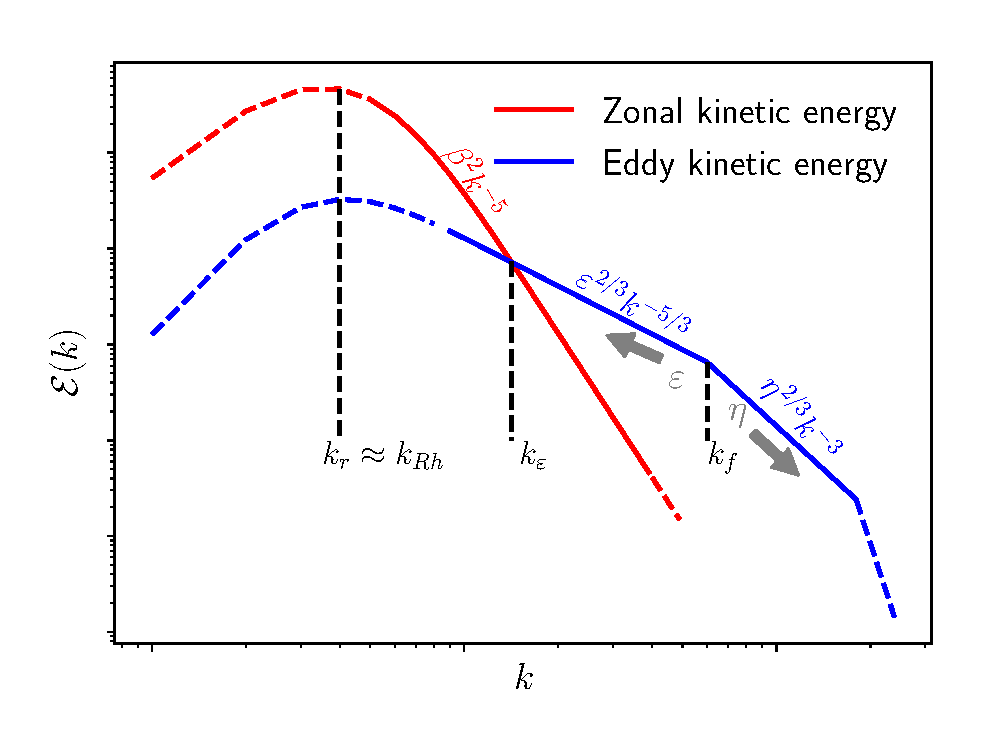
\includegraphics[width=4in]{EKE_ZKE_spectra_illustrate}\caption{Schematic illustration of kinetic energy spectrum in zonal modes (red
line) and eddies (blue) for the zonostrophic turbulence regime. Zonal
and eddy kinetic energy spectra intersect at the crossover wavenumber $k_{\varepsilon}$,
which is thought to be the boundary between near-isotropic turbulence and Rossby
waves. Inverse cascade is halted by friction at $k_{r}$, which is
close to the Rhines wavenumber $k_{Rh}$. The forcing is narrowly
centered at $k_{f}$.}
\label{EKE_KE_spectra_illustrate}
\end{center}
\end{figure}


\begin{figure}
\begin{center}
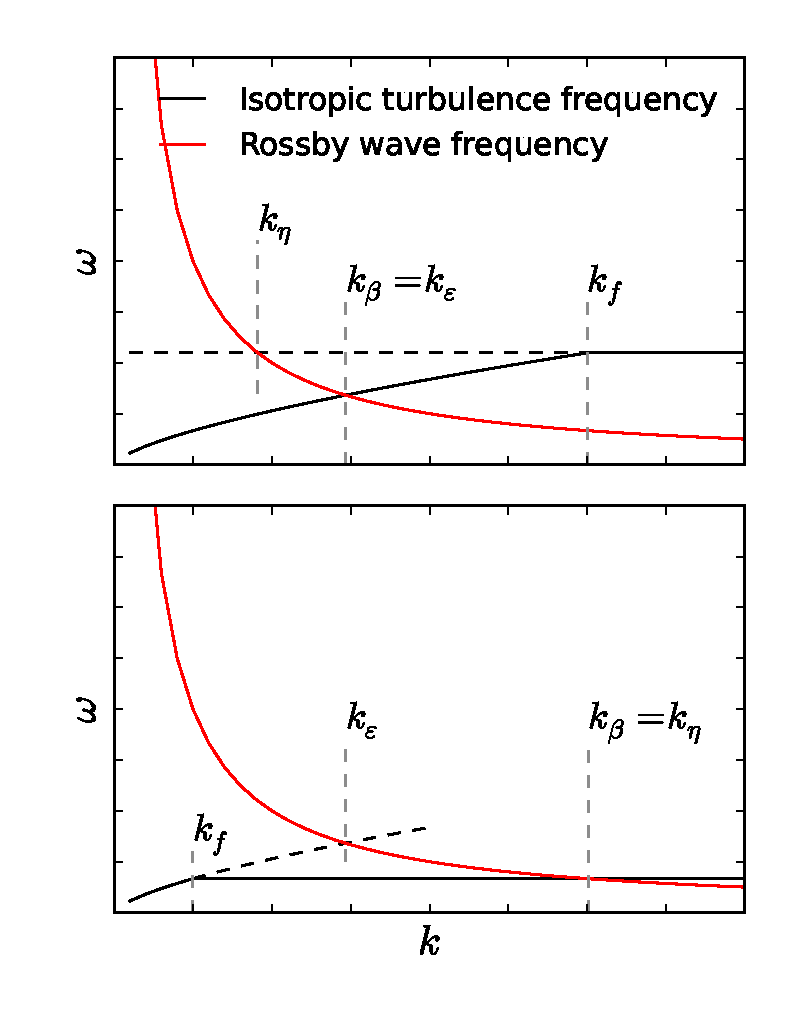
\includegraphics[width=4in]{crossover_scale_illustrate}\caption{Schematic illustration of isotropic turbulence frequency $\omega_{t}$
(black line) and Rossby wave frequency $|\omega_{\beta}|$ (red line).
$\omega_{t}$ and $|\omega_{\beta}|$ intersect (top) within the
inverse energy cascade range or (bottom) within the direct enstrophy
cascade range. The generalized turbulence-wave crossover wavenumber
$k_{\beta}$ is given by either $k_{\varepsilon}$ or $k_{\eta}$
depending on within which range $\omega_{e}$ and $|\omega_{\beta}|$ intersect.}
\label{crossover_illustrate}
\end{center}
\end{figure}


\begin{figure}
\begin{center}
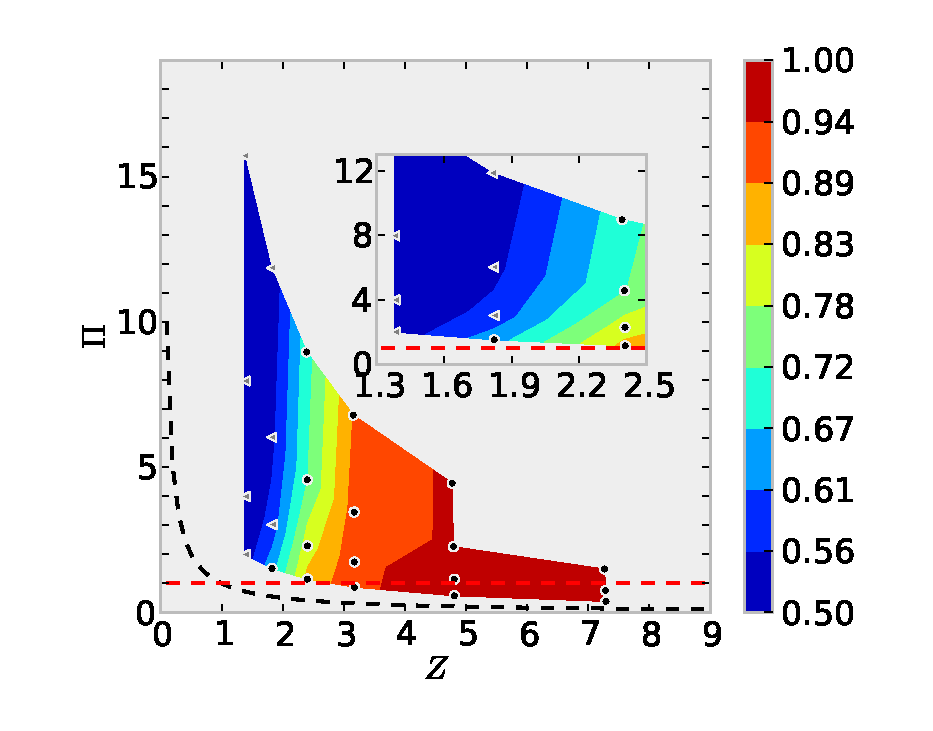
\includegraphics[width=6in]{anisotropic_index}\caption{Anisotropy index defined as $\chi=\langle u^{2}/(u^{2}+v^{2})\rangle$
in the $(Z,\Pi)$ space. The black dots indicate the runs in which
jets have formed, whereas the gray triangles donate runs that have
no clear visually identifiable jets. The inset is a zoom-in of the
region $Z\apprle2.5$.}
\label{anisotropic_index}
\end{center}
\end{figure}


\begin{figure}
\begin{center}
\includegraphics[width=6in]{vor_u_drag1024e-4}\caption{Snapshots of relative vorticity (left) and zonal velocity (right)
from $Z=1.8$ runs with $\Pi=$ (top) 1.5, (middle) 6.0, and (bottom)
11.9. The black line in the right panels denote zonal and time mean
zonal wind, with its axis in the bottom right subplot.}
\label{vor_u_snapshot_drag1024e-4}
\end{center}
\end{figure}


\begin{figure}
\begin{center}
\includegraphics[width=6in]{vor_u_drag256e-4}\caption{Snapshots of relative vorticity (left) and zonal velocity (right)
from $Z=2.4$ runs with $\Pi=$ (top) 1.1, (middle) 2.3, and (bottom)
9.0. The black line in the right panels denote zonal and time mean
zonal wind, with its axis in the bottom right subplot.}
\label{vor_u_snapshot_drag256e-4}
\end{center}
\end{figure}


\begin{figure}
\begin{center}
\includegraphics[width=6in]{vor_u_drag8e-4}\caption{Snapshots of relative vorticity (left) and zonal velocity (right)
from $Z=4.8$ runs with $\Pi=$ (top) 0.6, (middle) 1.1, and (bottom)
4.5. The black line in the right panels denote zonal and time mean
zonal wind, with its axis in the bottom right subplot.}
\label{vor_u_snapshot_drag8e-4}
\end{center}
\end{figure}


\begin{figure}
\begin{center}
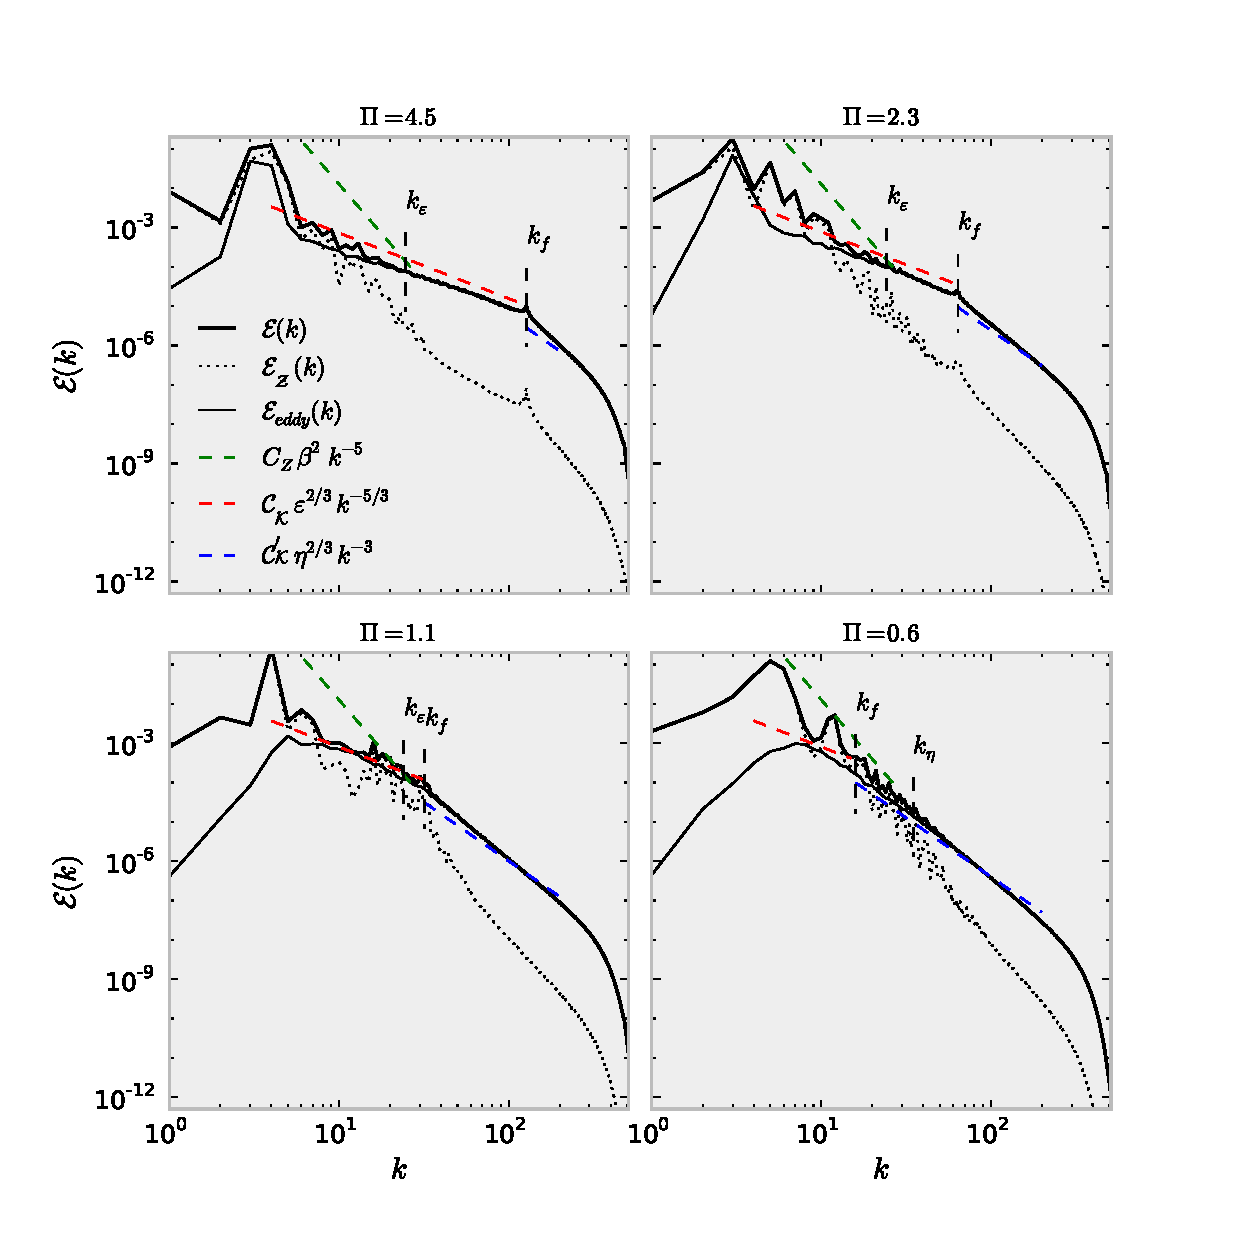
\includegraphics[width=6in]{E_ZKE_EKE_spectra_drag8e-4}\caption{The energy spectra of the total flow $\mathcal{E}(k)$ (thick solid
black line), eddies $\mathcal{E}_{eddy}(k)$ (thin solid black line)
and the zonal flow $\mathcal{E}_{\mathcal{Z}}(k)$ (dotted black line)
from simulations with $Z=4.8$ and various values of $\Pi$ varying
from 0.6 to 4.5 as indicated above the plots. The theoretical spectra
in energy and enstrophy cascade ranges are shown in red and blue dashed
lines respectively. The universal energy spectrum of the zonal modes
with $-5$ slope for zonostrophic turbulence regime is shown in green
dashed line.}
\label{E_EKE_ZKE_spectrum_drag8e-4}
\end{center}
\end{figure}


\begin{figure}
\begin{center}
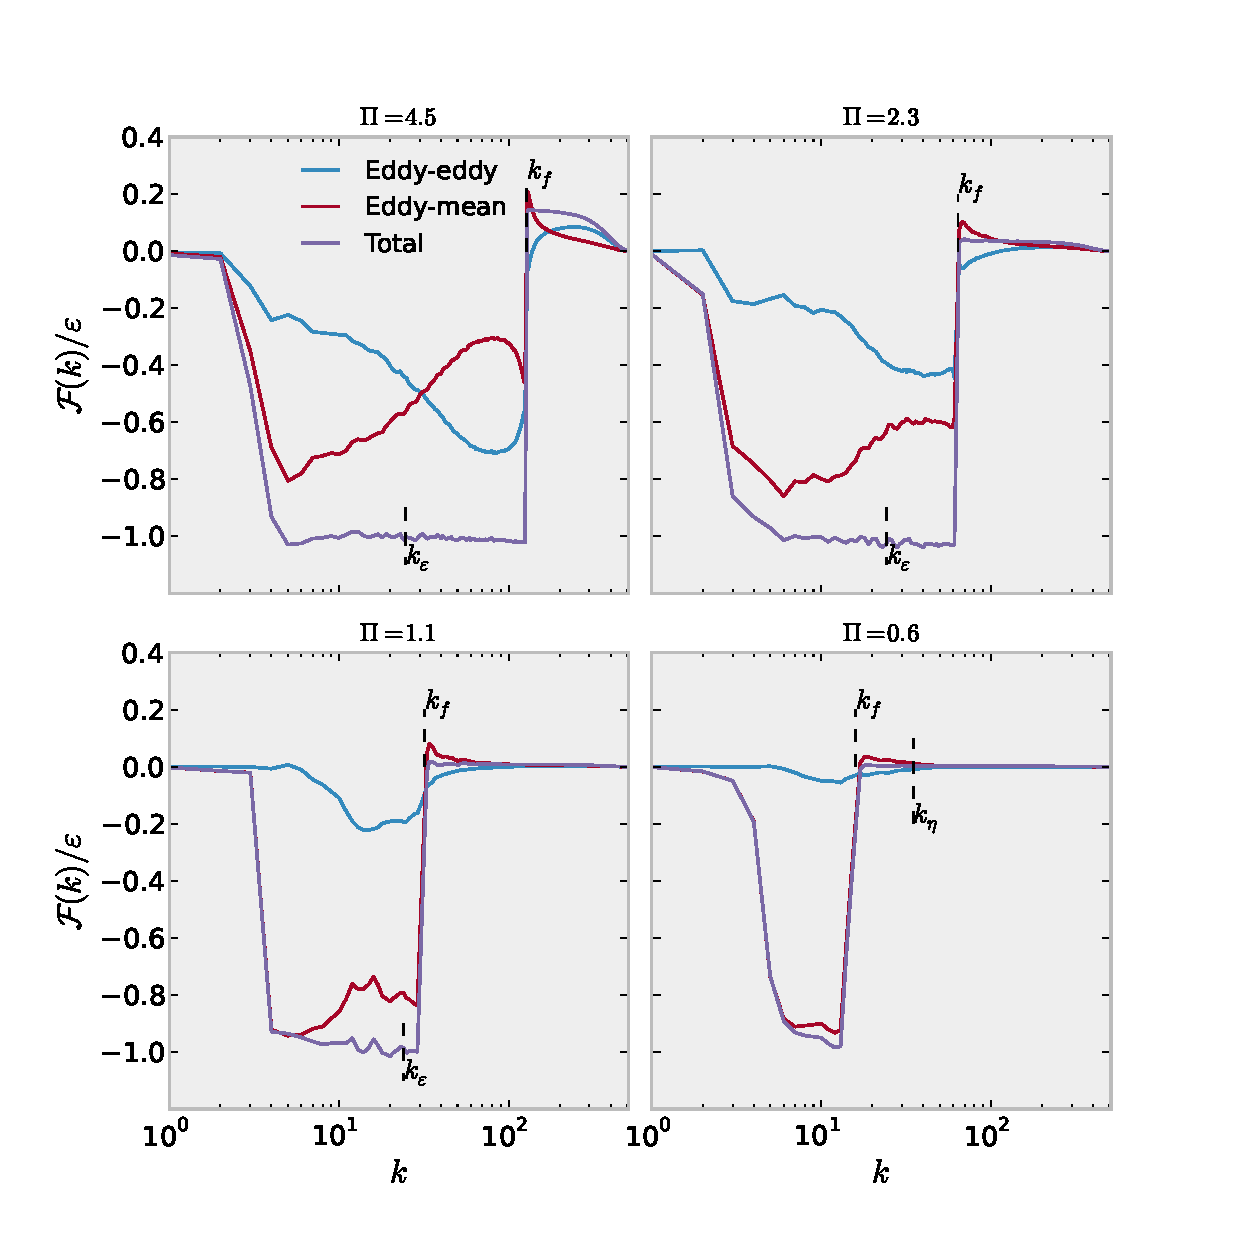
\includegraphics[width=6in]{NLflux_drag8e-4}\caption{Energy flux across wavenumber $k$ for simulations with $Z=4.8$ and
various values of $\Pi$. Energy flux of the total flow $F(k)$ is
the purple line, that of the eddy-eddy interactions $F_{EE}(k)$ is
the blue line, and that of the eddy/mean-flow interactions is the
red line.}
\label{energy_flux_drag8e-4}
\end{center}
\end{figure}


\begin{figure}
\begin{center}
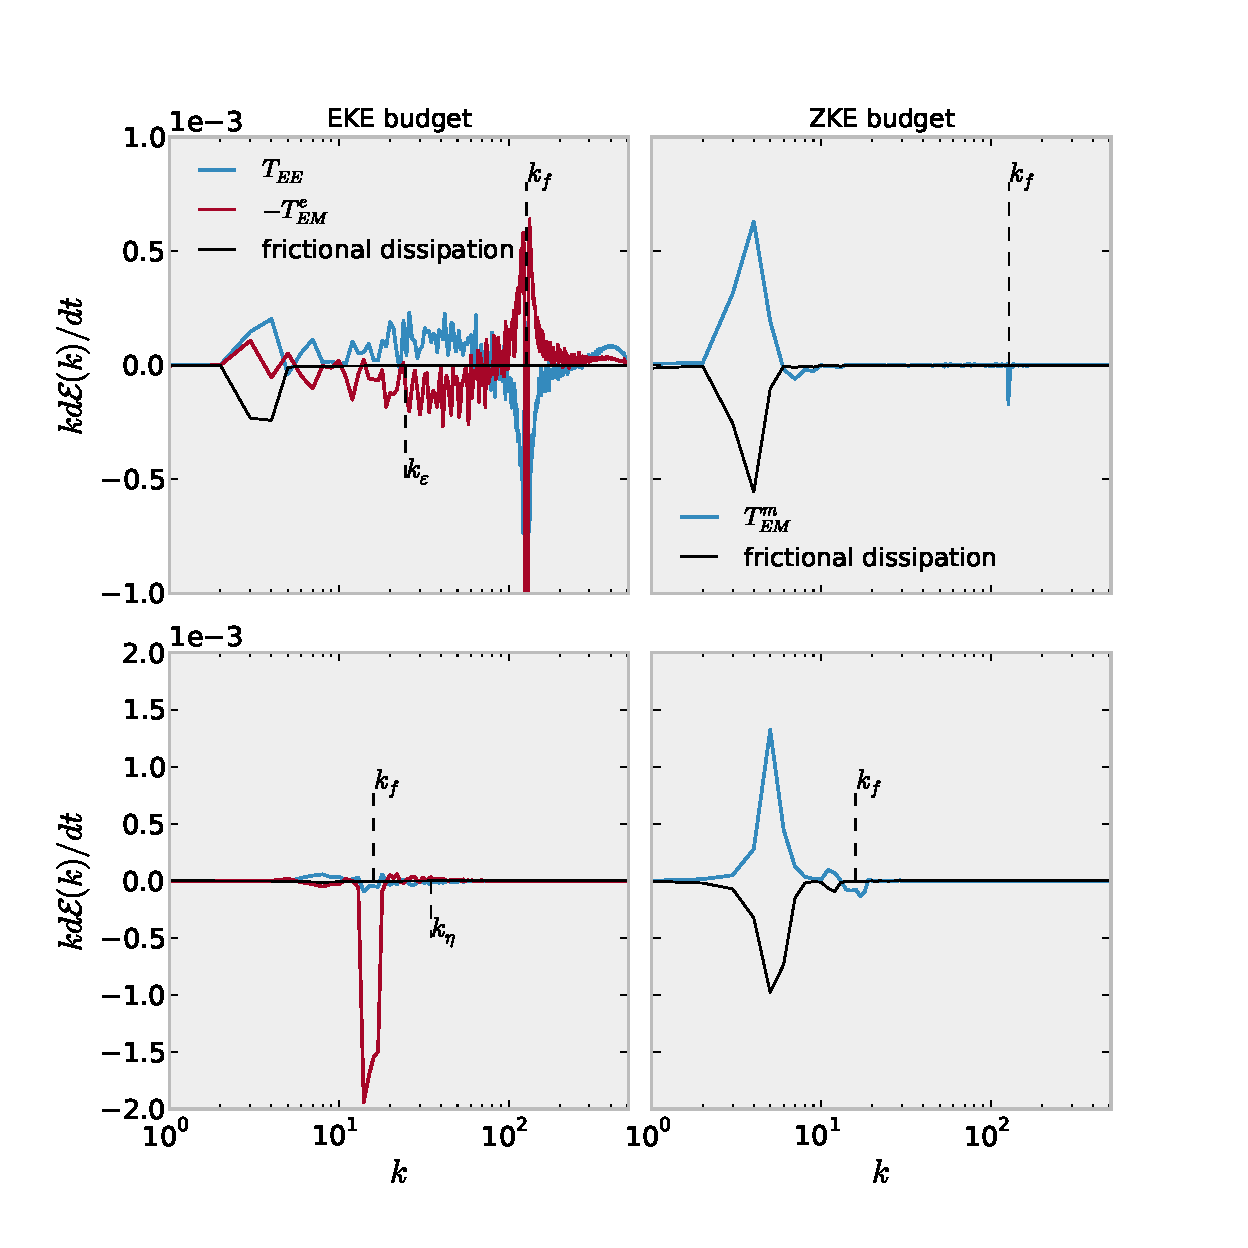
\includegraphics[width=6in]{EKE_ZKE_budget_drag8e-4}\caption{Spectral EKE and ZKE budgets for simulations with $Z=4.8$ and $\Pi=$(top)
4.5 and (bottom) 0.6. The formulation for these budgets are given
in (\ref{eq:EKE_spec_psi}) and (\ref{eq:spectral_ZKE_budget}).}
\label{EKE_ZKE_spectral_budget_drag8e-4}
\end{center}
\end{figure}


\begin{figure}
\begin{center}
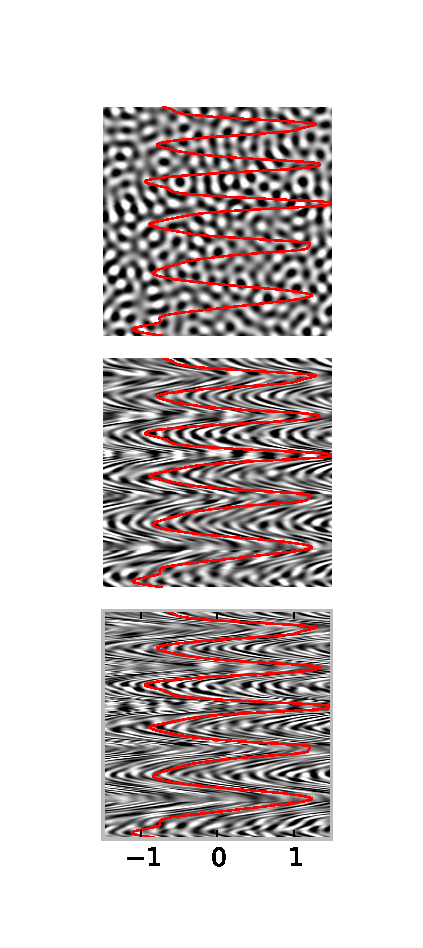
\includegraphics[width=3in]{eddy_vorticity_evolution}\caption{Snapshots of eddy relative vorticity at time $t=0$ (top), 0.78 (middle)
and 1.56 (bottom) from an initial-value run. The red lines denote
the zonal mean zonal wind, with its axis in the bottom subplot. The
parameters for this simulation is the same as $Z=4.8$ but without
forcing and friction. The initial condition is the time and zonal
mean flow from the simulation with $Z=4.8$ and $\Pi=0.6$ run with a
small-amplitude eddy perturbation, which is shown as eddy vorticity
field at $t=0$.}
\label{initial_value_run}
\end{center}
\end{figure}


\begin{figure}
\begin{center}
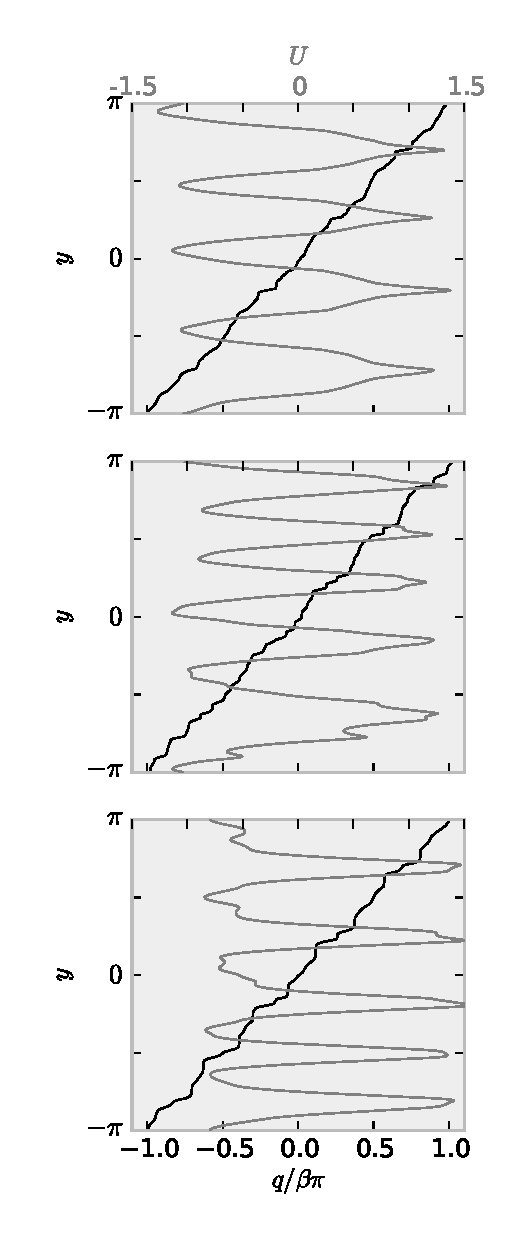
\includegraphics[width=3in]{PV_vs_y}
\caption{Zonal and time mean potential vorticity $\overline{q}$ (black line)
and zonal velocity $\overline{u}$ (gray line) from simulations with
$Z=7.3$ and $\Pi=$(top) 1.5, (middle) 0.76, and (bottom) 0.4. The
potential vorticity profile at equivalent latitude is almost indistinguishable
from $\overline{q}$, so it is not shown.}
\label{PV_vs_y_drag1e-4}
\end{center}
\end{figure}

\begin{figure}
\begin{center}
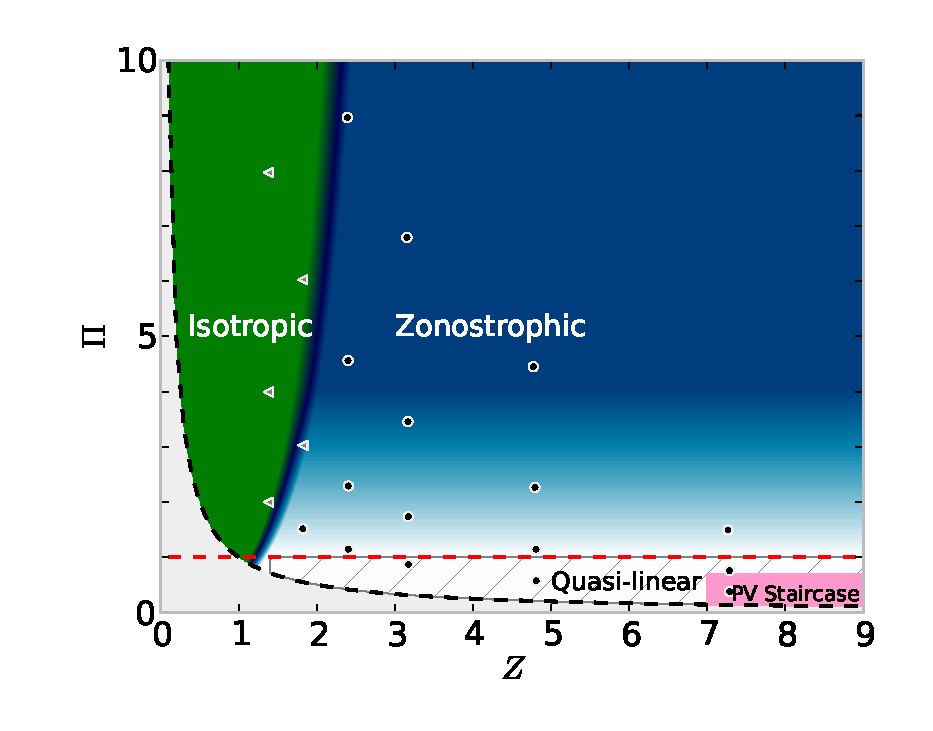
\includegraphics[width=4in]{regime_illustration}\caption{Chart of turbulence regimes in $(Z,\Pi)$ space.}
\label{regime_illustration}
\end{center}
\end{figure}



\end{document}
%%%%%%%%%%%%%%%%%%%%%%%%%%%%%%%%%%%%%%%%%%%%%%%%%%%%%%%%%%%%%%%%%%%%%
% END OF AMSPAPER.TEX
%%%%%%%%%%%%%%%%%%%%%%%%%%%%%%%%%%%%%%%%%%%%%%%%%%%%%%%%%%%%%%%%%%%%%